\documentclass[letterpaper,twocolumn,10pt]{article}
% Official USENIX FAST template (usenix2019_v3.sty), used 1:1. The style loads
% mathptmx (Times), fontenc, inputenc, microtype, hyperref, cite, url, xcolor and
% sets the 7in x 9in two-column block, so we add only graphicx/booktabs/amsmath.
% Double-blind: no author/affiliation (per FAST blindness policy).
\usepackage{usenix2019_v3}
\usepackage{graphicx}
\usepackage{booktabs}
\usepackage{amsmath}
\graphicspath{{figures/}}
% The template's own hypersetup colors citations red / links green on
% screen; override to plain black print-safe links, matching the accepted-
% paper convention and keeping the PDF anonymous.
\hypersetup{colorlinks=true, linkcolor=black, citecolor=black, urlcolor=black}

\title{Short Paper: Heaven's Eye: Self-Referential Addressing and Learned
Precoding for Glass Storage}
\author{}
\date{}

\begin{document}
\maketitle

\begin{abstract}
Flash wears out after a bounded number of program/erase cycles, magnetic media
must spin, and neither binds the bits it stores to the physical device holding
them.  We present \textbf{Heaven's Eye}, a rewritable optical block device built
from commodity glass, a fixed camera, and a small on-device neural codec.
Nothing moves, and no laser touches the glass.  Data lives in a reversible
optical state switched by light.  The glass's own manufacturing imperfections
serve as a coordinate frame that writer and reader both condition on and,
because that pattern is unique to each piece, as an intrinsic hardware key.  Heaven's Eye formulates write and read jointly as a deep joint
source-channel autoencoder trained through a differentiable optical channel,
with disorder maps drawn from 300 real optical-PUF speckle images.  A
0.17\,MB codec reads a simulated 16{,}384-cell, 64-block platter frame at raw
BER $6.5\times10^{-3}$ and recovers all 64 shuffled block identities by
imperfection fingerprint alone (\textbf{100\% addressing recovery}).  The
disorder is real; payload modulation and camera formation are calibrated
simulation.  A light-driven write on a coated coupon is the step from this
design to a built drive.
\end{abstract}

\section{Introduction}
Solid-state and magnetic drives are fast but imperfect: flash wears out after a bounded
number of program/erase cycles, both draw power to retain and serve data, and neither
carries an intrinsic physical identity binding stored bits to a specific piece of hardware.
Commodity glass has the opposite properties.  It is inexpensive, chemically inert,
and dimensionally stable, and it is never truly featureless: under the right
illumination every piece reveals a dense field of intrinsic imperfections, grains,
voids, scatterers, and variations in index and stress, unique to that piece. We ask whether a stable
commodity substrate, a camera, and on-device AI can be turned into a \emph{fast,
re-writable} storage device in the class of an SSD, with data read and written entirely by
light.

\textbf{Heaven's Eye} is that device: a fixed camera images a stationary commodity-glass
platter under electronically selected illumination, and an on-device AI model turns those
pictures into data and back.  Nothing moves, no laser or femtosecond source is
involved, and the glass itself is never physically modified.  Different light changes
what the camera sees, and that change is the I/O: the write path holds data in a
reversible, light-toggled state, switched by low-power illumination and read back by
the same camera.  Because the state is reversible and the substrate is never ablated,
the medium rewrites like an SSD.

Those imperfections carry no payload.  They play two other roles.  As a \emph{map},
enrolled once, they let the system address any cell relative to its neighbors rather
than by mechanical position.  As a
\emph{fingerprint}~\cite{pappu_puf_science02}, being random and unique to each piece,
they bind the stored bits to that physical substrate, giving a security key an SSD does
not have.

Heaven's Eye targets fast, re-writable read/write operation on glass, a different
framing of the medium from the prevailing write-once archival one.  We make three contributions.
\begin{enumerate}\itemsep2pt
\item \textbf{An imperfection-conditioned learned read/write codec}
(\S\ref{sec:codec}), in the deep joint source-channel
family~\cite{bourtsoulatze_deepjscc_tccn19}: a learned encoder (write) and a
FiLM-conditioned~\cite{perez_film_aaai18} decoder (read), trained jointly
through a differentiable optical channel.  To our knowledge this is the first
end-to-end \emph{learned write and read} for optical glass storage rather than a
learned decoder over a fixed write.  An ablation shows the conditioning is
load-bearing, not cosmetic: removing it raises BER from 0.13 to 0.40 at
4\,bits/cell.
\item \textbf{Self-referential addressing} (\S\ref{sec:landmarks}): the
medium's intrinsic imperfections used as a \emph{coordinate frame} rather than,
as in optical PUF work~\cite{pappu_puf_science02}, an identity.  This takes a
99.7\% open-loop registration failure rate to zero under drift, tilt, and
missing landmarks, and recovers the correct block order of a shuffled platter at
100\% accuracy, an LBA-style map keyed to the glass itself.
\item \textbf{A whole-platter, no-moving-parts read path} (\S\ref{sec:eval}): one
simulated frame over a real disorder map yields a 4{,}096-byte payload across 64 blocks
at BER $6.5\times10^{-3}$, roughly $166\times$ worse than the same codec's BER on the
synthetic sweep at matched bit-depth and signal level (\S\ref{sec:codec}), a real-vs-synthetic
disorder gap we return to in \S\ref{sec:eval}. The read path has a \emph{fixed}
$\approx$17\,ms modeled random-read latency with no seek term, and the reversible write's
modeled endurance crosses the ECC waterfall somewhere between 50 and 150 cycles, in
0.17\,MB and $\approx$0.38\,MFLOP/cell of codec compute.
\end{enumerate}

\section{Background: an SSD-class target}
We target the fast read/write tier occupied by SSDs and HDDs, not archival storage. The
relevant metrics are therefore random-access latency, rewrite endurance, areal density,
energy, cost, and, uniquely here, an intrinsic physical security key. Two properties of
the design set these. First, a single camera frame reads a whole region at once, so
random-read latency is one capture-plus-inference time (tens of milliseconds in our model),
set by optics and compute rather than any mechanical position. Second, data is held in a
reversible, light-toggled optical state, so rewrite endurance is a property of that optical
layer, not of charge-trap wear as in flash. On top of both, the glass's own imperfection
fingerprint supplies tamper-evidence and hardware binding at no extra cost. We quantify
these against SSD/HDD in \S\ref{sec:related}. Prior glass-storage
work~\cite{silica_sosp23,kazansky_5d_prl14} targets a different regime,
write-once archival with laser-written voxels, and is not our comparison point.

\section{Architecture: Camera, Light Actuator, and Compute}
\label{sec:arch}
Figure~\ref{fig:device} shows the device. A stationary multi-layer glass platter is
imaged by a fixed global-shutter monochrome CMOS sensor through macro/telecentric
optics under electronically selected wavelength, polarization, and coherence. The
pipeline is: illuminate, capture, calibrate, reconstruct, extract features,
ECC-decode, deliver host blocks over a PCIe/CXL host link; two modes, A (read-only
fingerprint) and B (reversible RW), share this pipeline,
differing only in whether the reversible optical state is set. A controller PCB, or in the
cheap instantiation an RPi-class SBC, ties glass, camera, illumination, and codec stages
together end to end (\S\ref{sec:model}).

\begin{figure}[t]\centering
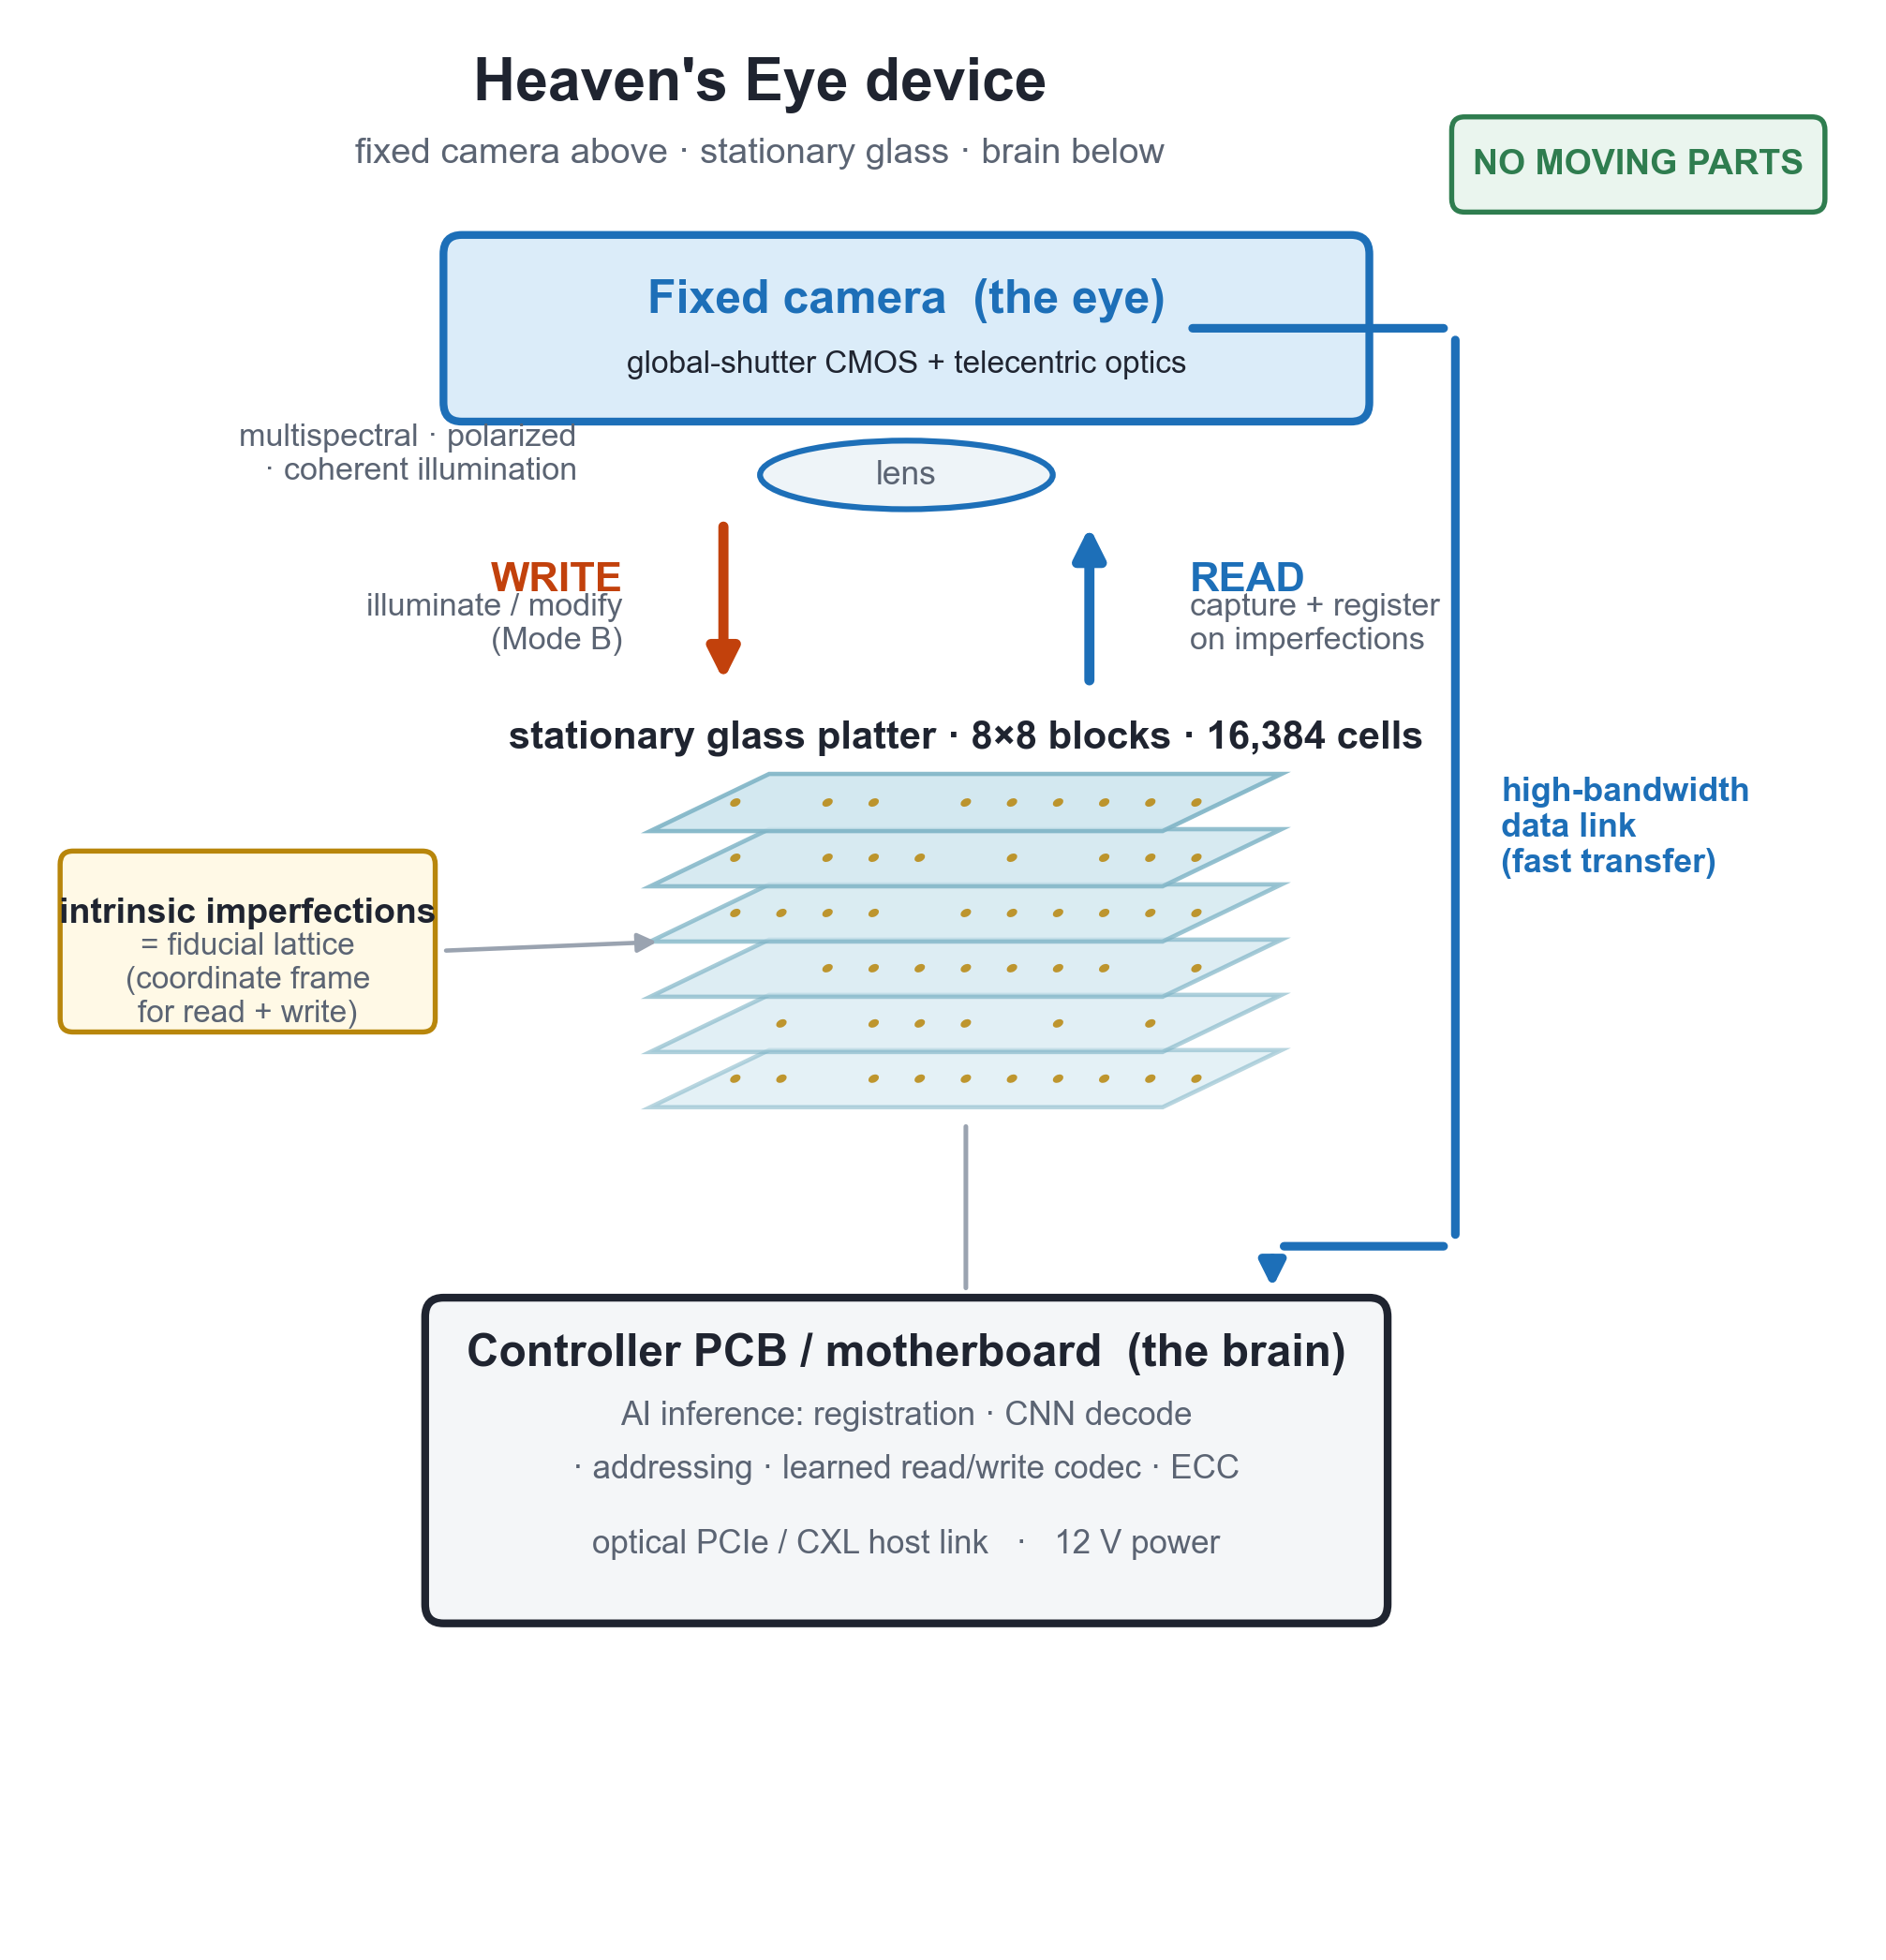
\includegraphics[width=0.8\columnwidth]{device.png}
\caption{Device: fixed camera, stationary glass platter, no mechanical scanning.}
\label{fig:device}
\end{figure}

\paragraph{Optical read and write on untouched glass.} A read is $R(G,S,L,C)$: the camera
image of the fixed intrinsic structure $G$ and a reversible optical state $S$, under
illumination $L$ and camera config $C$. The write sets $S$: a low-power, electronically
addressed light exposure toggles a reversible optical layer on the commodity glass (a
photochromic, thermochromic, or phosphorescent film) between distinguishable states, which
the layer holds after the light is removed. Nothing is carved, ablated, etched, or written
into the bulk glass, the substrate is untouched and reusable, and the stored change is a
reversible optical state the camera can see. This gives two modes on one reader (detailed next), sharing one camera, one
illumination controller, and one AI codec; there is no laser, no femtosecond source, and no
moving stage.

\paragraph{What is and is not written to the glass, two storage modes.}
\emph{Nothing is carved or etched into the bulk glass}. Storage takes one of two forms,
which we distinguish because they make different physical claims.
\emph{Mode~B, reversible-state write} (the mode our codec is trained on): a low-power light
exposure toggles a reversible optical layer between distinguishable states that persist after
the light is off. This is a real but reversible physical change, confined to a coating, not
the glass. It gives re-writable arbitrary-data capacity at the cost of a switchable film.
\emph{Mode~A, enrollment / map-to-imperfection} (no physical write at all): the glass's
fixed intrinsic imperfections are treated as a large, permanent random field, and ``storing''
data means committing a learned \emph{mapping} from imperfection features to payload bits.
Nothing on the glass changes; the decode key, the codebook plus the coordinate map, is
held in a small fast side-memory (RAM/NVRAM) in the controller, and readback re-images the
fixed field and applies that key. Mode~A costs zero write energy and yields an unmodifiable,
tamper-evident substrate and very fast reads (the key is in RAM), but its capacity is bounded
by the medium's fixed entropy and it is effectively write-once per enrollment; Mode~B adds
re-writability on top. In both modes a cell is found by \emph{self-referential addressing}, a ``GPS on the glass'': the enrolled imperfection lattice \emph{is} the coordinate frame, so
any location is fixed relative to nearby landmarks (\S\ref{sec:landmarks}), never by a
mechanical position or an external byte offset. Data is thus addressed \emph{to the
imperfections themselves}.

\paragraph{Light is the I/O channel.} Because the glass is never modified, all
information flows through how it is lit and imaged: dark-field illumination enrolls the
fingerprint lattice (\S\ref{sec:landmarks}), polarized illumination reads internal
stress/birefringence, and narrowband illumination at the reversible layer's absorption
peak both reads its switched state (low power) and writes it (high power, same band). The
change in appearance under light is the I/O.

\paragraph{Division of labor.} The on-device model is deliberately tiny per cell
(0.17\,MB, $\approx$0.38\,MFLOP/cell, \S\ref{sec:codec}), which makes a
fixed-function accelerator, rather than a datacenter GPU, a credible controller
target.  A full platter frame still costs 6.3\,GFLOP (\S\ref{sec:model}), beyond bare
RPi-class compute.  The camera and controller therefore handle capture, illumination
control, and registration locally; per-cell inference targets an accelerator; and ECC,
large-block encode/decode, and model retraining stream over the host link to host
CPU/GPU, exactly as an SSD controller offloads to its host.

\section{Model and Methodology}
\label{sec:model}
The simulator models media geometry (platter size, cell pitch, bits/cell), a fixed-camera
acquisition model (sensor MP, frame rate, reconstruction cost/Gpix), a camera-noise model
(full-well, read/dark noise, ADC quantization, modulation depth) yielding SNR/BER, and a
system model (capture/inference time, energy, no mechanical term). Noise and optics use
standard CMOS-sensor and microscopy constants; all values are model outputs
(``targets until measured''). The main sweep samples the per-site gain/offset
disorder; the platter experiment instead derives it from 300 images in the
public optical-PUF response set (Zenodo 8377156), training on a 2{,}400-patch
pool drawn from them.  In both cases \emph{the disorder is real, while payload
modulation and camera formation are simulated} (\S\ref{sec:codec}).

\paragraph{Compute efficiency of the on-device AI model.} The
``compact enough for an RPi-class board'' claim needs a real number, so we counted
parameters and multiply-accumulate operations directly from the implemented codec
(\S\ref{sec:codec}): 0.17\,MB total (43{,}121 parameters) at $\approx$39\,kFLOP/cell
encoder $+$ $\approx$344\,kFLOP/cell decoder ($\approx$0.38\,MFLOP/cell total),
sustaining millions of
cells/s on the GPU. We did not benchmark physical RPi hardware, so we
instead compare against published mobile-deployed models on structurally similar
problems as existing-precedent evidence: MobileNetV2 ($\approx$300\,MFLOPs, 3.4\,M
params, 72.0\% ImageNet top-1)~\cite{mobilenetv2_cvpr18}, MobileNetV3-Large
($\approx$219\,MFLOPs, 5.4\,M params, 75.2\%)~\cite{mobilenetv3_iccv19}, and
MobileFaceNets ($\approx$1\,M params, $\approx$450\,MFLOPs, 99.55\% LFW
accuracy)~\cite{mobilefacenets18}, all real-time on phone-class SoCs. Our codec is
$\approx$25--125$\times$ smaller by parameters and orders of magnitude cheaper per
inference (per cell vs.\ per image), comparative evidence, not a substitute for the
direct RPi measurement listed as a near-term step in \S\ref{sec:demo}.

\begin{figure}[t]\centering
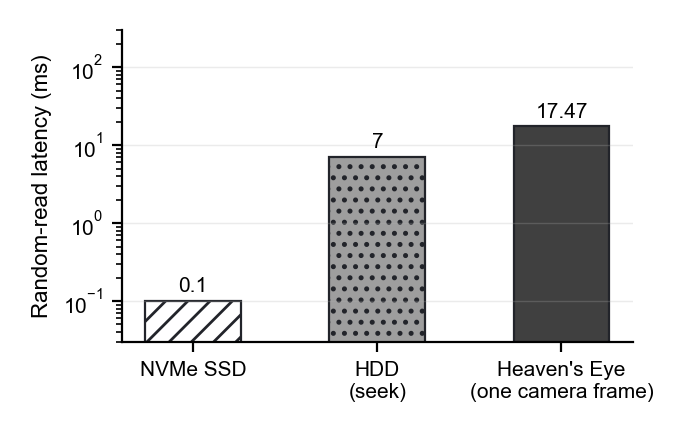
\includegraphics[width=0.8\columnwidth]{fig_latency_ladder.png}
\caption{Random-read latency vs.\ HDD and NVMe SSD (modeled).}
\label{fig:latency}
\end{figure}

\section{Learned Read/Write Codec}
\label{sec:codec}
We cast glass read/write as a \emph{learned channel autoencoder}, the deep joint
source-channel coding (JSCC) formulation of Bourtsoulatze et
al.~\cite{bourtsoulatze_deepjscc_tccn19}: a learned encoder maps data to channel inputs,
a fixed non-trainable channel sits in the middle, and a learned decoder recovers the
data, all trained jointly. Here the three pieces are physical. The \textbf{encoder}
(write) is a small CNN that maps a block of $M$-ary symbols, together with the local
intrinsic imperfection field, to a per-cell reversible modulation level in $[0,1]$, imperfection-aware \emph{precoding}. The \textbf{channel} is our differentiable optical
forward model: the modulation is applied \emph{relative to} a per-site imperfection field
(gain/offset, the intrinsic PUF/coordinate substrate~\cite{pappu_puf_science02}, write
mode~B), then blurred by the point-spread function (inter-symbol interference),
corrupted by Poisson shot and Gaussian read noise, quantized by the ADC
(straight-through), and illumination-calibrated. The \textbf{decoder} (read) is a
FiLM-conditioned~\cite{perez_film_aaai18} CNN equalizer that maps the camera image, again
conditioned on the imperfection field, to symbol logits. The imperfection field is thus a
\emph{shared} write/read side channel, consistent with \S\ref{sec:arch}: the codec never
writes the imperfections, it writes reversible modulation \emph{addressed against} them.
Training is SNR-adaptive, SNR is an input to both networks and randomized per step, so one model per bit-depth covers the whole SNR range. The decoder inherits the learned
optical-read-channel principle established for holographic
recording~\cite{nguyen_cnn_hds23} and production optical media~\cite{liu_decods26}, and
the FiLM-conditioned reconstruction shown for 5D glass~\cite{film_5d_storage_arxiv25}.

\begin{figure}[t]\centering
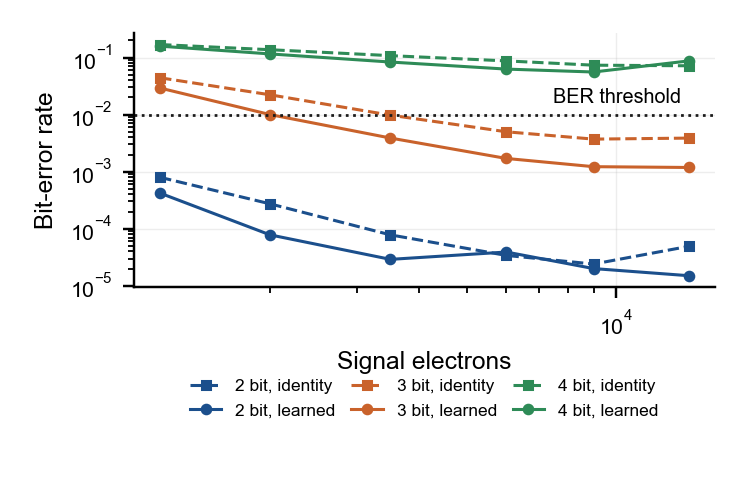
\includegraphics[width=\columnwidth]{rw_ber_snr.png}
\caption{Learned vs.\ identity write across bit-depth and SNR. Learned reaches the
waterfall at lower SNR (3 bits/cell).}
\label{fig:rwber}
\end{figure}

\paragraph{Learned write beats identity write (Fig.~\ref{fig:rwber}).} Across the sweep,
imperfection-aware precoding lowers BER versus an identity write (level $=$
symbol$/(M{-}1)$) paired with the same learned decoder: at 3 bits/cell the learned write
reaches BER 0.010 at 2000\,e$^-$, just above the $10^{-2}$ waterfall, and clears it by
3500\,e$^-$ (0.0039), while the identity write needs the full 3500\,e$^-$ to clear it
(0.0098, versus 0.022 at 2000\,e$^-$); it wins at 11 of 12 non-saturated operating points.
2 bits/cell stays below $10^{-4}$ for both above 3500\,e$^-$. Four bits/cell is
the hard frontier: neither write reaches the waterfall, and the shared SNR-adaptive
model is noisier there.

\paragraph{The imperfections are essential (ablation).} Removing the imperfection-field
conditioning from both encoder and decoder raises BER from 0.13 to 0.40 at the harder
4-bit/cell, 2600\,e$^-$ operating point (both above the waterfall; the platter result in \S\ref{sec:eval} runs at 2 bits/cell,
where this ablation has not been repeated). The
codec cannot equalize the channel without the field it wrote against, i.e.\ conditioning
is necessary side-information, not that the payload itself resides in the imperfections.

\paragraph{Rewritability and a working round trip.} Because the write is
reversible modulation, the medium is rewritable.  Under a contrast-fade model of
coating fatigue, BER sits below the $10^{-2}$ waterfall at 50 cycles (0.0039) and above
it by 150 (0.0186), with nothing sampled between, so the crossing falls somewhere in
that interval rather than at a value we can name.  This is endurance, not permanence,
and it is the price of rewritability.  A second, independent endurance model
(\texttt{sim/results/endurance.csv}) puts the crossing an order of magnitude higher,
entirely because the coating's decay-per-cycle is an unmeasured free parameter in both.
An
end-to-end bytes$\rightarrow$write$\rightarrow$camera$\rightarrow$read round trip at
2 bits/cell recovers a real 48-byte message at \textbf{100\% byte accuracy} (mean
decoder confidence 0.9997).

\begin{figure}[t]\centering
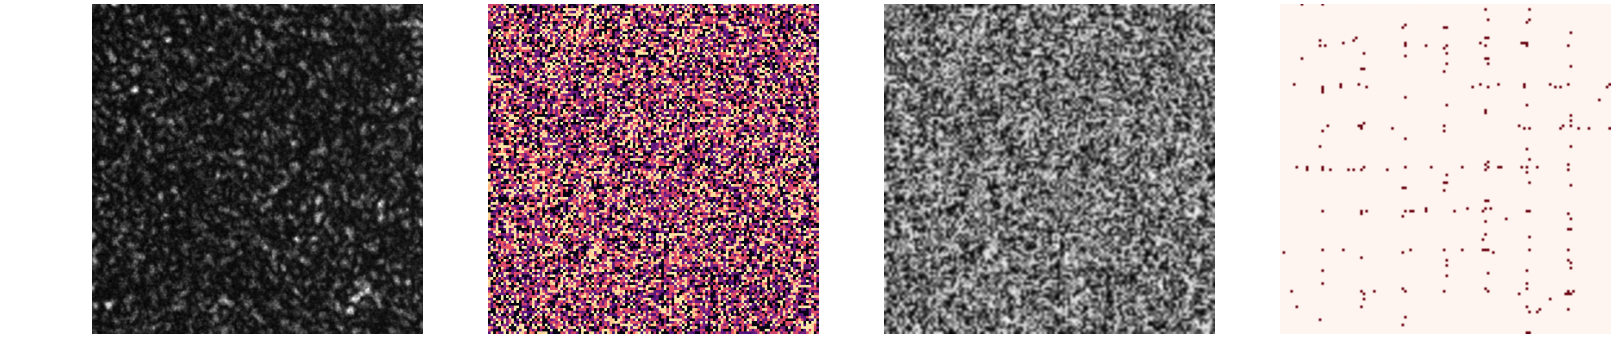
\includegraphics[width=\columnwidth]{whole_platter.png}
\caption{Whole-platter run over a real disorder map: imperfections, written payload,
simulated camera frame, decode errors (left to right). BER $6.5\times10^{-3}$.}
\label{fig:platter}
\end{figure}

\paragraph{Whole-platter operation: no wasted glass (Fig.~\ref{fig:platter}).} A real
reader images the whole platter in one frame, so the codec must use all of it, not a
single block. We tile one real disorder map into an
$8\times8$ grid of 64 addressable blocks (16{,}384 cells; a 4{,}096-byte payload at
2~bits/cell); the encoder writes a payload chunk into every block relative to \emph{that
block's own} imperfections, a single camera frame is \emph{simulated} over the full
platter (so blur crosses block seams), and the decoder re-tiles and reads every block. Whole-platter BER is
$6.5\times10^{-3}$ (95\% byte accuracy before ECC; per-block SER 0.013, rising to 0.031
only at seam blocks). Each block is addressed by its intrinsic-imperfection fingerprint:
shuffling the 64 blocks and matching each to the enrolled map recovers the correct order
at 100\% accuracy, an LBA-style block map keyed to the glass itself. The design thus
uses the medium's full information-bearing area, not a single demonstrated patch.

\paragraph{Stacking multiplies capacity (extension, not core).} Glass layers can
be stacked, each with its own imperfection field, and demixed by a learned decoder: a
\emph{focal stack} (one image focused per layer) holds mean BER below the $10^{-2}$
floor through four layers and a 3D voxel reconstruction matches the written field at
99.8\% accuracy at the sweep's highest tested signal level (14000\,e$^-$); a single
\emph{overlaid} snapshot already fails at $N{=}2$ (BER 0.17), so only the focal-capture
mode is viable. We treat multi-layer stacking as a secondary axis, not a claim of this
paper, and leave the full sweep (overlay-vs-focal, per-channel multiplexing,
decoder-capacity scaling) to an extended version.

\section{Evaluation}
\label{sec:eval}
\paragraph{Random-read latency (Fig.~\ref{fig:latency}).} A whole region is read in one
camera capture-plus-inference, $\approx$17\,ms in our model, with no mechanical position to
seek. That is slower than an SSD ($\sim$0.1\,ms) and comparable to an HDD seek
($\sim$5--10\,ms), but it is a \emph{fixed} cost independent of access pattern, and it is
paid by optics and compute rather than a moving head; the whole-platter pipeline
(\S\ref{sec:codec}) amortizes it across an entire snapshot of many blocks.

\paragraph{Capacity/throughput frontier and BER vs.\ SNR.} These evaluations model the
fixed-camera read channel across cell pitch, bits/cell, and SNR (down to 0.5\,$\mu$m cells),
bounding areal density and reliability from a single snapshot; the reversible layer's
density and endurance are the subject of \S\ref{sec:demo}.

\paragraph{Energy.} A single reader delivers $\approx$3.9\,MB/s/W in the streaming limit
versus $\approx$875\,MB/s/W for NVMe: glass does not win the streaming-per-watt race, but it
draws no standby power to retain data and needs no mechanical actuation, and the write is a
low-power light exposure rather than charge programming.

\paragraph{Honest workload fit.} Fast, no-moving-parts random reads ($\approx$17\,ms)
with a re-writable optical state and a built-in hardware fingerprint fit
\emph{re-writable secure storage and tamper-evident working sets}, where hardware
binding matters and rewrite counts are moderate, rather than write-once archival or
the highest-churn hot paths where SSDs win, a judgment from the endurance and
addressing numbers rather than a benchmarked result.

\section{Self-Referential Addressing via Intrinsic Microstructure}
\label{sec:landmarks}
A fixed-optics reader has no mechanical stage, so the hard problem is not motion but
\emph{registration}: under drift, tilt, thermal expansion, and vibration, where is a
given data cell in the captured frame? Our answer is to make the medium
self-referential. Real glass (and ceramic, and similar substrates) is full of stable
intrinsic imperfections: grains, voids, bubbles, scatterers, index variations.
Enrolled once as a reference map, these form a dense fiducial lattice; at each access,
the system registers the observed landmark constellation to the map (a least-squares
affine fit tolerating missing/noisy landmarks) and addresses each cell \emph{relative
to its neighboring imperfections}. The same coordinate system doubles as the write
channel's conditioning side-information (\S\ref{sec:codec}): the reversible write
(\S\ref{sec:arch}) is addressed and precoded against it, so rewrite and verify are
repeatable at the same location.

We test this with a Monte Carlo model (cell pitch $=1$): enroll random landmarks,
apply an unknown affine distortion plus per-landmark noise and missing landmarks,
register, and measure residual localization error (Table~\ref{tab:landmarks}).
Open-loop (no landmarks) fails at a 99.7\% error rate (residual $\sim$5.7 cells under
8-cell drift); 80 landmarks over a $200\times200$-cell field drop the error rate to
\emph{zero} under that same mild condition (Table~\ref{tab:landmarks}). A separate,
denser sweep (2{,}000 landmarks, the same 0.05/cell density) holds sub-cell accuracy
even under a much harsher 60-cell drift, 10$^\circ$ tilt, and 60\% missing landmarks;
the 80-landmark density itself remains untested under that harsher condition.

\begin{table}[t]\centering\small
\setlength{\tabcolsep}{4pt}
\caption{Landmark addressing: residual localization error and addressing-error rate
vs landmark density (noise 0.15 cell, 8-cell drift, 2$^\circ$ tilt, 1\% scale, 20\%
missing). Model results, median over 40 seeds.}
\label{tab:landmarks}
\begin{tabular}{rrrr}
\toprule
Density & Landmarks & Median err & Addr.\ error \\
(/cell) & (200$^2$) & (cells) & rate \\
\midrule
0.000 & 0 & 5.68 & 0.997 \\
0.002 & 80 & 0.038 & 0.000 \\
0.010 & 400 & 0.017 & 0.000 \\
0.050 & 2{,}000 & 0.008 & 0.000 \\
0.250 & 10{,}000 & 0.003 & 0.000 \\
\bottomrule
\end{tabular}
\end{table}

\paragraph{Write-then-verify closes the loop.} Because a cell is addressed
relative to the same imperfections at write and read time, write and verify agree
whenever their two registrations agree to within a cell. In a marginal regime, a
single write-once pass leaves 8.1\% of cells failing verification.  A Mode~B retry loop
re-attempts a failed write within the same logical write operation, rather than
rewriting already-good data, and drives delivered write errors to 0.9\%, 0.05\%, and
0.006\% after one, two, and three retries (Table~\ref{tab:rw}).  Retries are not free:
if a logical write costs up to three of them, the effective write count is a fraction of
the raw cycle budget.  That raw budget crosses the ECC waterfall between 50 and 150
cycles, with the caveats of \S\ref{sec:codec}; true endurance remains a materials
measurement (\S\ref{sec:demo}).

\begin{table}[t]\centering\small
\setlength{\tabcolsep}{6pt}
\caption{Write-then-verify on the landmark frame (marginal regime). Model results,
40 seeds.}
\label{tab:rw}
\begin{tabular}{lr}
\toprule
Policy & Delivered write-error rate \\
\midrule
Single-pass (no rewrite) & 0.081 \\
Mode B (1 rewrite) & 0.0088 \\
Mode B (2 rewrites) & 0.0005 \\
Mode B (3 rewrites) & 0.00006 \\
\bottomrule
\end{tabular}
\end{table}

\section{Related Work}
\label{sec:related}

\paragraph{Positioning against SSD/HDD.}
Table~\ref{tab:systems} places Heaven's Eye against SSD and HDD, not archival media. An
HDD pays a mechanical seek per random read; an SSD wears out after a bounded
program/erase budget; neither ties stored bits to the physical part. Heaven's Eye reads a
whole region in one camera frame (latency set by optics and inference, not a head),
rewrites via a reversible optical state, and architecturally binds data to the substrate
via imperfection fingerprints (unevaluated, \S\ref{sec:limits}). The costs are areal
density and latency (tens of ms, slower than an SSD); all device numbers are
calibrated-simulation and real-image results pending \S\ref{sec:demo}.

\begin{table}[t]\centering\small
\setlength{\tabcolsep}{4pt}
\caption{Heaven's Eye vs.\ the fast read/write tier. SSD/HDD figures are typical vendor
characteristics; Heaven's Eye figures are calibrated-simulation / real-image outputs
(\S\ref{sec:eval},\S\ref{sec:codec}), not measured hardware.}
\label{tab:systems}
\setlength{\tabcolsep}{3pt}
\resizebox{\columnwidth}{!}{%
\begin{tabular}{llll}
\toprule
 & HDD & SATA SSD & \textbf{Heaven's Eye} \\
\midrule
Random read & 5--10\,ms & $\sim$0.1\,ms & $\approx$17\,ms (one frame) \\
Moving parts & yes (heads) & none & \textbf{none} \\
Rewritable & yes & yes (limited P/E) & yes (optical cycles) \\
Wear mode & mechanical & charge-trap P/E & coating fatigue \\
Fingerprint mechanism$^\dagger$ & no & no & \textbf{yes} \\
Medium & magnetic & NAND flash & commodity glass + coating \\
\bottomrule
\end{tabular}}
\end{table}
\vspace{-2pt}
{\footnotesize $^\dagger$Architectural property only; we run no adversarial, cloning,
or multi-piece evaluation (\S\ref{sec:limits}).}

Prior glass storage, including Project
Silica~\cite{silica_sosp23,silica_tos25,silica_nature26} and the 5D
nanostructuring line it builds on~\cite{kazansky_5d_prl14,wang_100layer_lpr22},
targets write-once archival with femtosecond-laser voxels read by a robotic
mount; we target the warm, re-writable tier, so that work places our design
rather than competing with it. Optical PUFs showed that a camera can digitize a
disordered medium's microstructure into stable bits~\cite{pappu_puf_science02};
we build on this, using that microstructure as a shared read/write coordinate
frame and hardware fingerprint.
Learned ISI cancellation is established in adjacent optical channels: CNN equalizers correct
2D interference in holographic recording~\cite{nguyen_cnn_hds23}, and a learned optical read
channel decodes past the diffraction limit on production media~\cite{liu_decods26}; a
FiLM-conditioned network reconstructs 5D nanostructured-glass
states~\cite{film_5d_storage_arxiv25}. Our delta is specific: those decoders
learn to read a \emph{fixed} physical write, whereas our encoder is learned too,
so write and read are co-designed; and we condition on the medium's
\emph{intrinsic disorder} rather than on a laser-written state, which is what
turns the imperfections from a nuisance into a coordinate frame. We know of no prior
work using a disordered medium's own imperfections as the shared read/write coordinate
frame for a re-writable optical device. Computational microscopy (Fourier
ptychography~\cite{fourier_ptychography13}, dark-field and polarized imaging) established
motion-free wide-field imaging, letting a fixed camera address the platter without a scan
stage. Mobile-deployed CNNs~\cite{mobilenetv2_cvpr18,mobilenetv3_iccv19,mobilefacenets18}
establish sub-gigaflop, high-accuracy pattern recognition on phone-class hardware, the
same problem class as decoding glass microstructure; \S\ref{sec:model} gives the
per-model numbers our decoder beats on both metrics, the basis for our RPi-class
compute claim.

\section{What We Demonstrate, and the Remaining Physical Step}
\label{sec:demo}
\paragraph{Provenance.} The full codec is trained and evaluated end to end through the
differentiable channel, every artifact committed. Calibrated-synthetic: conditioning is
essential ($0.40\!\rightarrow\!0.13$), the learned write beats a naive write, and a
round trip recovers a short message at 100\% byte accuracy. Real optical-disorder:
4{,}096 bytes across 64 blocks at 95\% byte accuracy. All learned results are
single-seed; \S\ref{sec:limits} sets out the held-out-glass and multi-seed gap.

\paragraph{The one remaining physical step.} What the GPU demonstration cannot supply
is the materials measurement: how a real reversible layer on real glass behaves under a
real light write. \texttt{REAL\_WORLD\_TEST.md} specifies a turnkey, low-cost
($<$\$60) coupon test, a commodity glass slide with a reversible light-responsive
layer, an LED write light, and a phone camera, with falsifiable success criteria
(post-registration BER $<10^{-2}$, $\geq$10 rewrite cycles, $\geq$2 decodable
illumination channels), feeding the resulting images straight back into the same
codec. No coupon results exist yet; that single measurement, not the architecture,
is what remains open.

\paragraph{Deployment and resilience.} The device is a host-attached module: camera
and controller do capture, illumination, and registration; per-cell inference
(6.3\,GFLOP/platter-frame at $\approx$17\,ms, \S\ref{sec:model}) needs a fixed-function
accelerator rather than a bare RPi-class CPU, and ECC and large-block coding run on the
host. Striping across cells, blocks, and platters makes losing one platter a recoverable
erasure, as RAID tolerates a failed disk, and the intrinsic fingerprint is designed to
make a swapped platter distinguishable on re-enrollment, a capability we describe but
have not adversarially tested (\S\ref{sec:limits}). This complements rather than
competes with write-once archival glass, which stores cold data for centuries with a
laser.

\section{Limitations}
\label{sec:limits}
\textbf{The light-driven write has not been experimentally validated on a physical
coated coupon, by us or, to our knowledge, by anyone in this form.} All learned
results are single-seed, and training and evaluation draw from the same 300-image disorder
pool rather than a held-out split; both are single-run gaps a revision closes with reported
confidence intervals. All device numbers are calibrated-simulation and real-image outputs
(turnkey test, \S\ref{sec:demo}) and could differ once measured; the write's spatial
resolution is coarser than the read resolution, setting an unmeasured density ceiling, and
throughput-per-watt trails NVMe.
Evaluating a new medium in a calibrated model, validating physically as a separate step,
follows the DNA archival store~\cite{dna_asplos16} and Pelican~\cite{pelican_osdi14}. The
fingerprint mechanism is architectural, not evaluated: the 64-block addressing test matches
crops of one disorder map against themselves, with no inter-piece, adversarial, cloning, or
aging result, so Table~\ref{tab:systems}'s fingerprint row is an unevaluated capability.

\section{Conclusion}
Heaven's Eye reads data on commodity glass relative to the glass's own imperfections,
a shared write/read coordinate map. A jointly-trained encoder/decoder pair reads a
simulated platter frame over a real disorder map at BER $6.5\times10^{-3}$ in a
0.17\,MB model. A coated-coupon experiment is the next step toward validating the
complete physical write path.

\section*{Data Availability}
Heaven's Eye's codec, channel simulator, and every committed result artifact are
available at \url{https://github.com/ttad22/HEyE}. Disorder maps are drawn unmodified
from the public optical-PUF set, Zenodo record 8377156.

\bibliographystyle{abbrv}
\bibliography{refs}

\end{document}
